\documentclass[10pt, compress]{beamer}

\usetheme{m}

\usepackage{booktabs}
\usepackage[scale=2]{ccicons}
\usepackage{minted}

\usemintedstyle{trac}

\title{A Hybrid Matchmaking Engine Using Advanced Recommender System }
\subtitle{Under the guidance of Dr. Pramod Kumar Singh}
\date{\today}
\author[shortname]{K. Shashank (2014IPG-47)\and\\ P. Akhilesh Naik (2014IPG-111)\and\\ Jk. Snehith (2014IPG-121) }
\institute{ABV INDIAN INSTITUTE OF INFORMATION TECHNOLOGY AND MANAGEMENT}

\begin{document}

\maketitle

\begin{frame}[fragile]
  \frametitle{MOTIVATION}
  \begin{itemize}
 \item<1> Why we choose this topic ?
 \item<1> Recommendation systems in  e-commerce.
\end{itemize}
\end{frame}

\begin{frame}[fragile]
  \frametitle{Introduction}
  \begin{itemize}
  \item<1> Defining recommender system.
  \item<1> Content based, Collaborative filtering
 \item<1> A glance of Proposed recommender system.


 \end{itemize}
\end{frame}

\begin{frame}[fragile]
  \frametitle{Objective} 
  \begin{itemize}
   \item<1> The objective of the following study is to bring contribution to the efficiency of recommender systems used in matrimonial sites that are well used in online dating sites in other parts of world 
   \item<1> Enable users to get their match in a more accurate way using content based scoring algorithms and reciprocal recommendations.
   \item<1> To solve the cold-start problems by being able to provide recommendations immediately based on new user's profiles and preference. 
   \item<1> In the later part we use  collaborative filtering which uses the interactions of the similar active users, including the people they like/dislike and are liked/disliked by, to result in recommendations.
 \end{itemize}
\end{frame}

\section{Literature Review}

\begin{frame}{Literature Review}
\transboxin
\small
\begin{tabular}{|p{1in}|p{3.2in}|}
 \hline
 \bf  contributors & \bf Features \\
  \hline
  {\center{Recon systems}} & \begin{itemize}\setlength\itemsep{0.02em} {\item Combination of content-based RS and reciprocal algorithm \item User profile and interactions with other user as parameters - implicit preferences\item Matching with complementary profiles}
  \end{itemize}\\
  \hline
{\center{Brozosky, petricek}} & \begin{itemize}\setlength\itemsep{0.02em}{\item Two recommender systems developed based on collaborative filtering }\end{itemize}\\
\hline
\end{tabular}
\end{frame}

\begin{frame}{ Literature Review}
\transboxin
\small
\begin{tabular}{|p{0.8in}|p{3.2in}|}
 \hline
 \bf  contributors & \bf Features\\
 \hline
{\center{K. Joshi and S. Kumar }} & {\begin{itemize}\setlength\itemsep{0.0em}{\item Use of AHP in matrimony to calculate weights of different attributes}
\end{itemize}}\\
\hline
{\center{Sampath.M.K}} & {\begin{itemize}\setlength\itemsep{0.0em}{\item Use of collaborative filtering in matrimonial sites}\end{itemize}}\\
  \hline
 {\center{ S. Khavate and M. A. Potey}} & {\begin{itemize}\setlength\itemsep{0.0em}{\item Use of partial fuzzy scoring system for indian matrimony}\end{itemize}}\\
 \hline
\end{tabular}
\end{frame}

\section{ matrimonial site and domain overview }

\begin{frame}[fragile]
  \frametitle{Matrimonial site}
  \begin{itemize}
 \item<1> The matrimonial site - Its intent, purpose  and the requirement of the user.\\~\
 \item<1> Creates a profile for himself/herself or the person for whom he/she would want to find a match.\\~\
 \item<1> User's Profile are further divided into \alert{account information, contact information, personal profile and preferred partner's profile}.\\~\
 \item<1> Following the completion of user profile now partner preferences are taken respectively. On completion the user becomes an \alert{active user} of the site.\\~\
 \item<1> The preferred partner profile consist of user's excepted range of age, range of height, range of income, religion, caste, education, occupation, complexion, body-type, diet, smoke and drink.\\~\
 
 
 \end{itemize}
 \end{frame}
 
 \begin{frame}[fragile]
  \frametitle{Matrimonial site cont\ldots}
  \begin{itemize}
  \item<1> Now recommendations are given to the active user based on the partner's preferences.\\~\
 
 
 \item<1> Some of the attributes preferences may have \alert{null values}.
 \end{itemize}
\end{frame}

\begin{frame}[fragile]
  \frametitle{Domain overview} 
 \begin{figure}[h!]
    \centering
    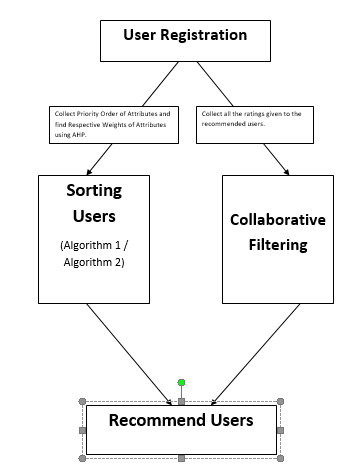
\includegraphics[width=0.6\textwidth]{images/flow.PNG}
    \label{fig:flow}
\end{figure}
\end{frame}



\section{The concept of AHP}

\begin{frame}[fragile]
  \frametitle{Analytic Hierarchy Process}
  \begin{itemize}
  \item<1> Complex multi-criteria decision making framework \\~\
  \item<1> \alert{HOW IT WORKS?}
 \item<1>Pair-wise comparison\\~\
 \item<1> \alert{MAKING COMPARISON MATRIX}
  \item<1> Pair-wise comparisons are analyzed
  \item<1> Spectrum of values from (1 to 9) and  (\(\displaystyle \frac{1}{9} \) to  \(\displaystyle \frac{1}{2} \)) are available
  \item<1> $A_i_j$ = 1/$A_j_i$
 \end{itemize}
\end{frame}

\begin{frame}[fragile]
  \frametitle{Analytic Hierarchy Process cont\ldots}
  \begin{itemize}
  \item<1> \alert{PRIORITY AND EIGEN VECTORS}
  \item<1> Normalized eigen vector is known as priority
  \item<1> Each value in the matrix is divided by the sum its column.
  \item<1> Normalized eigen vector is obtained by Averaging the rows.
  \item<1> 
 \end{itemize}
\end{frame}

\begin{frame}[fragile]
  \frametitle{}
  \begin{itemize}
 \item<1> \alert{HOW TO COMPUTE AHP IN FULL HIERARCHY }\\~\
 \begin{figure}[h!]
    \centering
    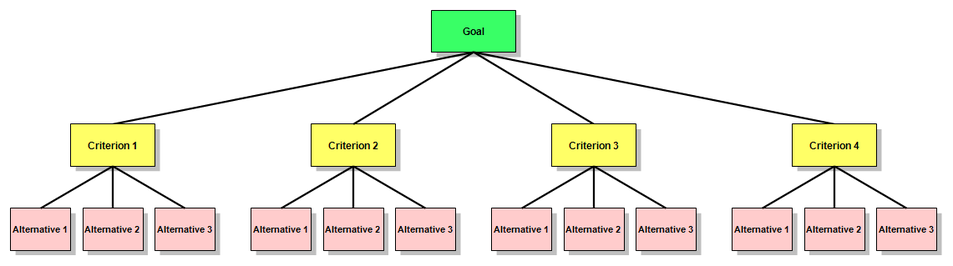
\includegraphics[width=0.8\textwidth]{images/AHP.png}
    \caption{AHP HIERARCHY}
    \label{fig:AHP}
\end{figure}
$W_i$=  $W_i$’ * W\textsubscript{PriorNode}
 \end{itemize}
\end{frame}

\begin{frame}[fragile]
  \frametitle{Use of AHP in Our Algorithm}
Algorithm takes the the priority order of  the user as $a , b , c , d $  which technically mean $ a > b > c > d $ then the corresponding comparison matrix of size $ 4 x 4 $ is as follows : 
\end{frame}

\begin{frame}[fragile]
  \frametitle{}
   \begin{figure}[h!]
    \centering
    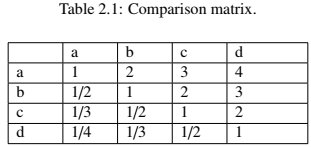
\includegraphics[width=0.8\textwidth]{images/Capture_1.png}
\end{figure}
corresponding weights:\\
$Weight_a = 0.46$ , $weight_b = 0.27$ , $weight_c = 0.15$ , $weight_d = 0.09$
\end{frame}

\section{Scoring Algorithm-1}

\begin{frame}[fragile]
  \frametitle{Scoring Algorithm-1 \ldots}
  \begin{itemize}
  \item<1> Classification of attributes into High important and Low important groups
  \item<1> High importance attributes: \alert{Religion, Caste, Occupation, Diet, Smoke, Drink}
  \item<1> Low importance attributes: \alert{Age, Height, Education, Income, Body Type Complexion}
  \item<1> Shortlisting of recommendations
  
 \end{itemize}
\end{frame}

\begin{frame}[fragile]
  \frametitle{Scoring Algorithm-1 \ldots}
  \begin{equation*}
    Similarity Index(SI) = 1-dist * factor
  \end{equation*}
  \begin{itemize}
  \item<1> \alert{dist} is distance between preference and profile value
  \item<1> \alert{factor} = 1/no of possible values for that attribute\\
  \item<1> For example, if user \alert{A}'s \alert{Complexion} preference is \alert{Wheatish}
   \begin{equation*}
   factor = 1/4 = 0.25
  \end{equation*}
  \end{itemize}
\end{frame}
\begin{frame}{fragile}
  \frametitle{Scoring Algorithm-1 \ldots}
\begin{itemize}
\begin{figure}[h!]
    \centering
    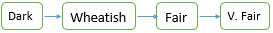
\includegraphics[width=0.7\textwidth]{images/algo1.PNG}
    \label{fig:algo1}
\end{figure}
  \begin{table}
    \caption{SI of complexion attribute for user A}
    
    \begin{tabular}{ccc}
      \toprule
      User & Complexion & Similarity\\
       \midrule
      C & Wheatish & 1-0=1\\
      B & Dark & 1-1*0.25=0.75\\
      D & Fair & 1-1*0.25=0.75\\
      E & Very Fair & 1-2*0.25=0.5\\
     \bottomrule
    \end{tabular}
  \end{table}
   \item<1> Calculating SI for all \alert{Low} importance attributes
    \end{itemize}
\end{frame}



\begin{frame}[fragile]
  \frametitle{Scoring Algorithm-1 \ldots}
  \begin{equation*}
    Score = \sum_{i=1}^{6} similarity_i * weight_i
  \end{equation*}
  \begin{itemize}
  \item<1> Recommendations in the descending order of scores
  \end{itemize}
\end{frame}

\section{Scoring Algorithm-2}



\begin{frame}[fragile]
  \frametitle{}
   Here firstly we intake 
  \begin{itemize}
	\item<1>User Profile\\~\
	\item<1>User Preferential List
	  \begin{itemize}
	      \item\textbf{ Most Preferred}: Diet: Vegetarian
	      \item\textbf{ Preferred}: Diet: Eggitarian
	      \item\textbf{ Least Preferred}: Diet:  Non Vegetarian
	  \end{itemize}\\~\
	\item<1>User Priority Order\\~\
	\item<1>Order of Criteria

 \end{itemize}
\end{frame}

\begin{frame}[fragile]
  \frametitle{User profile}
   \begin{figure}[h!]
    \centering
    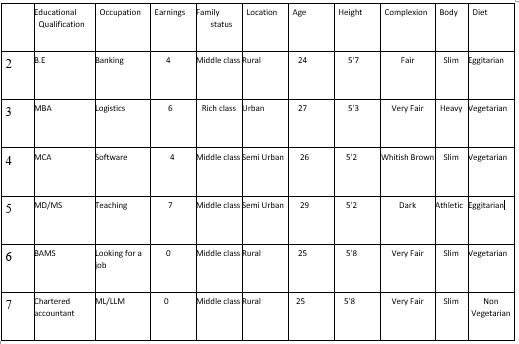
\includegraphics[width=0.8\textwidth]{images/table2.PNG}
    \caption{User Profiles}
    \label{fig:table2}
\end{figure}
\end{frame}

\begin{frame}[fragile]
  \frametitle{User Preferential List}
  \begin{itemize}
      \begin{figure}[h!]
    \centering
    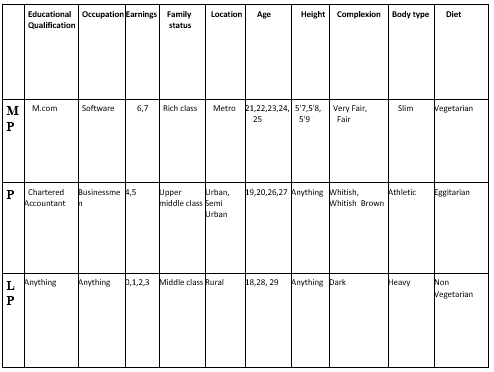
\includegraphics[width=0.8\textwidth]{images/table1.PNG}
    \caption{User Preferential List}
    \label{fig:table1}
\end{figure}
 \end{itemize}
\end{frame}

\begin{frame}[fragile]
  \frametitle{User priority order and Order of Criteria\ldots}
  \begin{figure}[h!]
    \centering
    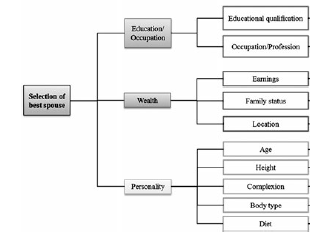
\includegraphics[width=0.6\textwidth]{images/Capture.png}
    \caption{HIERARCHY OF ATTRIBUTES}
    \label{fig:AHP}
\end{figure}
\begin{itemize}
\item<1>(Education,Wealth,Personality)
 \item<1> Educational Qualification,Occupation,Earnings,Family status,Location,Age,Height,Complexion,Body type,Diet
\end{itemize}
\end{frame}


\begin{frame}[fragile]
  \frametitle{scoring algorithm 2 cont\ldots}
  \alert{Levels are introduced}
  \begin{itemize}
\item<1> Level 1 (1, 100, 10000)
\item<1> Level 2 (1, 10, 100)
\item<1> Level 3 (1, 4, 16)
\item<1> Level 4 (1, 2, 4)

 \end{itemize}
\end{frame}

\begin{frame}[fragile]
  \frametitle{scoring algorithm 2 cont\ldots}
  Level  X (1, $\alpha$, $\beta$)\\~\
\begin{itemize}
\item<1>  If Value(i\textsubscript{bride}) = Value (i\textsubscript{bridegroom}) in\\~\
\item<1> \textbf{Most Preferred Category} : $ Score_i$ = $\beta$ * $W_i$ 
\item<1> \textbf{Preferred Category} : $ Score_i$ = $\alpha$ * $W_i$
\item<1> \textbf{Least Preferred} : $ Score_i$ = 1 * $W_i$
\begin{equation*}
    Score = \sum_{i=1}^{10} score_i
  \end{equation*}
\end{itemize}\\~\

\end{frame}

\begin{frame}[fragile]
  \frametitle{scoring algorithm 2 cont\ldots}
  \begin{itemize}
  \item<1>\alert{ Level 1 (1, 100, 10000)}
 \item<1> Most Preferred (MP)
 \item<1> \alert{ Level 2 (1, 10, 100)}
 \item<1> Most Preferred + Best(Preferred)
 \item<1> \alert{ Level 3 (1, 4, 16)}
 \item<1>Most preferred + Better(Preferred) + Best(Least Preferred)
 \item<1> \alert{ Level 4 (1, 2, 4)}
 \item<1> MP + Almost(Preferred) + Better(Least Preferred)
 
 
 \end{itemize}
\end{frame}

\begin{frame}[fragile]
  \frametitle{scoring algorithm 2 cont\ldots}
  \begin{itemize}
  \item<1>'Age': 0.06, 'Family status': 0.08, 'Body type': 0.016, 'Diet': 0.01, 'Height': 0.04, 'Educational Qualification': 0.35, 'Complexion': 0.02, 'Location': 0.04, 'Occupation': 0.17, 'Earnings': 0.16
  \begin{table}
    \caption{Sample scores of candidates}
    \begin{tabular}{cccc}
      \toprule
  & User 1 & User 2 & User 3\\
       \midrule
      MP & Diet & 0 & 0\\
\hline
P & 0 & 10 & EQ\\
\hline
LP & 9 & 0 & 9\\
     \bottomrule
    \end{tabular}
  \end{table}
 \item<1> Level 1: 1 > 2 > 3
 \item<1> Level 2: 2 > 1 > 3
 \item<1> Level 3: 2 > 3 > 1
 
  \end{itemize}
\end{frame}

\begin{frame}[fragile]
  \frametitle{scoring algorithm 2 cont\ldots}
   \begin{equation*}
   (Satisfatory factor)_i  = a_i/b_i
   \end{equation*}
  \begin{itemize}
  \item<1>$a_i$ = Max (No. of liked users in interval I , No. of disliked users in the interval I)
 \item<1> $b_i$ = Min (No. of liked in the interval I , no. of disliked users in the interval I)
 \item<1> i = interval
 \item<1> \Sigma $(satisfatory factor)_i$ > 0
  \end{itemize}
  \begin{figure}[h!]
    \centering
    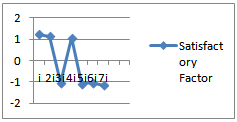
\includegraphics[width=0.6\textwidth]{images/graph.PNG}
    \label{fig:graph}
\end{figure}
  \end{frame}

\section{Collaborative Algorithm}
\begin{frame}[fragile]
  \frametitle{Collaborative Algorithm \ldots}
  \begin{itemize}
  \item<1> Generating similar users based on user preferences
  \item<1> Generating candidates to be considered for recommendation based on user interaction
  \item<1> Assigning scores to candidate users
 \end{itemize}
\end{frame}

\begin{frame}[fragile]
  \frametitle{Generating similar users}
  \begin{itemize}
 \begin{figure}[h!]
    \centering
    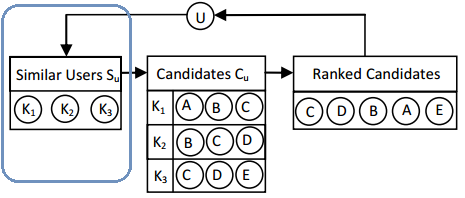
\includegraphics[width=0.6\textwidth]{images/ppt31.png}
    \label{fig:ppt31}
\end{figure}
\item<1> A list of K most similar users $S_u$ to $U$ in active user's gender group
\item<1> Based on distance metrics
\item<1> Fill the list with users whose preferences are similar to active user
 \end{itemize}
\end{frame}

\begin{frame}[fragile]
  \frametitle{Generating candidate users}
  \begin{itemize}
 \begin{figure}[h!]
    \centering
    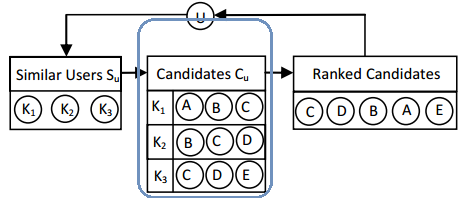
\includegraphics[width=0.6\textwidth]{images/ppt32.png}
    \label{fig:ppt32}
\end{figure}
\item<1> Candidates in unordered fashion
\item<1> Reciprocal interest
\item<1> For every user in similar users list ($S_u$), we retrieve the all the users that he/she has reciprocal interest with
 \end{itemize}
\end{frame}

\begin{frame}[fragile]
  \frametitle{Scores to candidate users}
  \begin{itemize}
 \begin{figure}[h!]
    \centering
    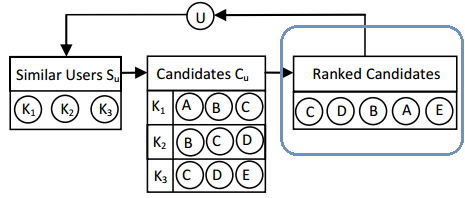
\includegraphics[width=0.6\textwidth]{images/ppt33.png}
    \label{fig:ppt33}
\end{figure}
\item<1> A candidates might have received positive interest from more than one $S_u$ user (multiple reciprocity)
\item<1> For each candidate user $X$  in the candidate list, we calculate the number of times $X$ has a positive interaction with a user in similar list $S_u$
\item<1> Similarly negative interaction
\item<1> Score = #positive - #negative
 \end{itemize}
\end{frame}

\begin{frame}{fragile}
  \frametitle{continued \ldots}
  \begin{table}
    \caption{Sample scores of candidates}
    \begin{tabular}{cccc}
      \toprule
Candidate & Positive responses & Negative responses & Score\\
       \midrule
      A & 2 & 7 & -5\\
\hline
B & 6 & 5 & 1\\
\hline
C & 12 & 6 & 6\\
\hline
D & 6 & 2 & 4\\
     \bottomrule
    \end{tabular}
  \end{table}
   \begin{itemize}
   \item<1> Higher the score, more he is liked reciprocally
   \item<1> Recommended in the descending order of scores
    \end{itemize}
\end{frame}
\section{Results and Discussion}

\begin{frame}{fragile}
  \frametitle{Scoring Algorithm 1 \ldots}
 \begin{itemize}
 \item<1> Implementation of algorithm on sample data 
   \item<1> The LOW importance preferences of a prospective bride is as follows:  age - 24 to 26, height - 5.9 to 6, education - Diploma, annual income - 8 lakhs  to 10 lakhs., body type - Average, complexion - Wheatish.
    \end{itemize}
  \frametitle{continued \ldots}
\begin{table}[h!]
\caption{Profiles of active bride grooms}
\vspace{0.1in}
 \begin{tabular}{|c|c|c|c|c|c|c|c|c|c|c|c|c|}
 \hline
 U-ID & Age & Height  & Education  & Income & Body & Complexion\\
 \hline
 21 & 26 & 5.7  & Masters & 4L & Athletic & Dark\\
 \hline
 22 & 24 & 5.5  & Doctors & 7L & Slim & Dark \\
 \hline
 23 & 30 & 5.1 & Doctors  & 14L & Avg & Wheatish \\
 \hline
 24 & 22 & 4.10 & HSC & 8L & Avg & Fair\\
 \hline
 25 & 26 & 5.2 & Bachelors & 3L & Hvy & VFair\\
 \hline
\end{tabular}
\end{table}\\
  
\end{frame}

\begin{frame}{fragile}
  \frametitle{Scoring Algorithm 1 \ldots}
 \begin{itemize}
 \item<1> Users are recommended in the decreasing order of scores
    \end{itemize}
  \frametitle{continued \ldots}
\begin{table}[h!]
\centering
\caption{Recommendations for Active Bride}
\vspace{0.1in}
 \begin{tabular}{|m{3cm}|m{2em}|}
 \hline
 User-ID & Score\\
\hline
21 & 49.3\\
\hline
24 & 48.4\\
\hline
22& 46.45 \\
\hline
23 & 40.2 \\
\hline
25 & 44.65 \\
\hline
\end{tabular}
\end{table}
  
\end{frame}

\begin{frame}[fragile]
  \frametitle{Continued \ldots}
  \begin{itemize}
  \item<1> \alert{Level 1}:  \[3 > 4 > 6 > 5 > 7 > 2\]
  \item<1> \alert{Level 2}:  \[3 > 4 > 7 > 5 > 2 > 6\]
  \item<1> \alert{Level 3}:  \[3 > 4 > 7 > 2 > 5 > 6\]
  \item<1> \alert{Level 4}:  \[3 > 4 > 7 > 2 > 5 > 6\]
 \end{itemize}
\end{frame}
\section{Conclusion}

\begin{frame}
Our partially developed algorithm have shown that the two proposed recommender systems not only gives a new way of gaining information from users but also explains the mutual acceptance by providing matches with much similarity between them and not only are we providing N-recommendations but the order of each match that is provided to active user is taken into account, its an improvement in the field known less important.

\end{frame}

\plain{}{Thank you }

\end{document}
